%!TEX TS-program = xelatex 
%!TEX TS-options = -output-driver="xdvipdfmx -q -E"
%!TEX encoding = UTF-8 Unicode
%
%  seminar_1
%
%  Created by Mark Eli Kalderon on 2010-01-17.
%

\documentclass[11pt]{article} 

% Definitions
\newcommand\myauthor{Mark Eli Kalderon} 
\newcommand\mytitle{Empiricism and the Philosophy of Mind}
\newcommand\mysubtitle{Parts I and II}

% Packages
\usepackage{url}
\usepackage{txfonts}
\usepackage{color}
\definecolor{myblue}{rgb}{0.8,0.8,1}

% Define discussion environment
\makeatletter\newenvironment{discussion}{%
   \noindent\begin{lrbox}{\@tempboxa}\begin{minipage}{\columnwidth}\setlength{\parindent}{1em}}{\end{minipage}\end{lrbox}%
   \colorbox{myblue}{\usebox{\@tempboxa}}
}\makeatother

% XeTeX
\usepackage[cm-default]{fontspec}
\usepackage{xltxtra,xunicode}
\defaultfontfeatures{Scale=MatchLowercase,Mapping=tex-text}
% \setmainfont{Palatino}
\setmainfont{Hoefler Text}
\setmonofont{Inconsolata}

% Title Information
\title{\mytitle\\
\mysubtitle}
\author{\myauthor} 
\date{} % Leave blank for no date, comment out for most recent date

% PDF Stuff
\usepackage[plainpages=false, pdfpagelabels, bookmarksnumbered, backref, pdftitle={\mytitle}, pagebackref, pdfauthor={\myauthor}, xetex, colorlinks=true, citecolor=gray, linkcolor=gray, urlcolor=gray]{hyperref}

%%% BEGIN DOCUMENT
\begin{document}

% Title Page
\maketitle

% Layout Settings
\setlength{\parindent}{1em}

% Main Content

\begin{figure}[htbp]
	\centering
		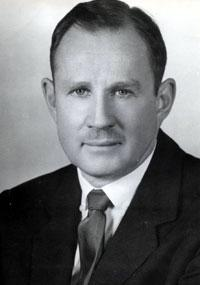
\includegraphics[scale=0.5]{../graphics/sellars.jpeg}
	\caption{Wilfrid Sellars}
	\label{fig:sellars}
\end{figure}

\section{An Ambiguity in Sense-Datum Theories} % (fold)
\label{sec:an_ambiguity_in_sense_datum_theories}

\textbf{Section 1}: Sellars aims to attack ``the whole idea of givenness,'' but proposes to do so by beginning with a special case---the given as it arises in sense-datum theories. Sellars doesn't explicitly tell us what the given is. No doubt he assumed that his audience at the University of London Special Lectures in Philosophy in March of 1956 knew, at least approximately, what he meant by the given. Whatever the merits of that assumption, it is less likely to be the case for us now. Instead, we must rely on the scattered clues provided by the text.

In attacking the given, Sellars doesn't mean to undermine the distinction between ``\emph{inferring} that something is the case and, for example, \emph{seeing} it to be the case''. Notice the distinction is between inferring and propositional seeing, seeing-\emph{that}. And since seeing is marked out as just an example, if a prominent one, the distinction is presumably between judgements formed on the basis of inference and non-inferential judgments paradigmatically (if not inevitably) formed on the basis of perception. ``The given'' is meant to carry ``substantial theoretical commitments'' that go beyond this commonplace.

\textbf{Section 2}: Sellars sketches the framework of the classical sense-datum theory. He focuses on the act--object structure that sense-datum theorists attribute to sensings understood as conscious episodes. On the one hand, there is the act of awareness or \emph{sensing}, and on the other hand there is the object of that awareness, the \emph{sense content}. % Thus Moore in sensing the blue bead, we can distinguish the act of awareness---Moore's sensing, and what Moore was aware of---the sense content of that awareness (which presumably includes the bead's shape and color).
The act of awareness involved in sensory experience may or may not be further analyzable (this will be relevant in §4).

In addition, Sellars makes the suggestion that different sense modalities (visual sensing, tactual sensing, etc.) may be distinguished by their sense contents (as opposed to positing distinct kinds of sensings.) This is controversial given that there are sense contents available to distinct sensory modalities (we can see a shape and feel it---or at least this is an alternative left open by Molyneaux's question to Locke).

\textbf{Section 3}: What's the ontological status of sense contents? Are they facts or particulars? This forms the basis of a dilemma:
\begin{enumerate}
	\item It is \emph{particulars} which are sensed. Sensing is not knowing. The existence of sense-data does not \emph{logically} imply the existence of knowledge.
	\item Sensing \emph{is} a form of knowing. It is \emph{facts} rather than \emph{particulars} which are sensed.
\end{enumerate}

Notice so far in Sellars' discussion all that is in play of the sense-datum theory is the act--object structure of sensing and the (plausible if optional) hypothesis that the objects of sensings are particulars. Both claims can and have been endorsed by philosophers who are not themselves sense-datum theorists. One prominent historical example with which Sellars was undoubtedly familiar is early Prichard (at least prior to 1921 with ``Seeing Movements''). Early Prichard ascribes to \emph{perception} (if not experience) an act--object structure and insists that the objects of perception are particulars. So Sellars' dilemma for the sense-datum theorist is applicable to other positions as well. So not only is Russellian acquaintance a target here, but so is Cook-Wilsonian apprehension.

Sellars remarks that on the first alternative sensing a sense content (where sense contents are particulars) is a \emph{non-epistemic} fact. This is important since, as we shall see, the Myth of the Given is claimed to be analogous to Moore's naturalistic fallacy. Just as Moore claimed that it was a mistake to infer normative truths from (non-normative) natural truths, Sellars claims that it is a mistake to infer epistemic truths from non-epistemic truths. So what's an ``epistemic fact'' here? It is at least clear that facts about a subject's knowledge count as epistemic facts. So it is an epistemic fact about me that I know, say, that there was an earthquake in Haiti. So being about a subject's states of propositional knowledge is \emph{sufficient} for a fact to be epistemic. Perhaps it is also the case that epistemic facts always involve propositional states of a subject. Are states of a subject's propositional knowledge not only sufficient but necessary for being epistemic? Or would propositional states of a subject that aren't knowledge states (such as nonfactive attitudes like justified belief) count as epistemic. For the most part this won't matter since Sellars' focus will be on the non-propositional character of sense data.

According to Sellars, ``the epistemological category of the given is, presumably, to explicate the idea that empirical knowledge rests on a `foundation' of non-inferential knowledge of matter of fact''. Moreover, Sellars seems to think that if the given is to play this role, the given must entail epistemic facts---specifically, facts about the subject's non-inferential knowledge. Why is that in order for the given to play this epistemological role it must \emph{entail} non-inferential knowledge? Why must the sense in which the given \emph{grounds} non-inferential knowledge be wither identity or entailment (as opposed to some suitable explanatory relation)?

\textbf{Section 4}: Sellars suggests that the sense-datum theorist can have their cake and eat it to. The way to do so is to understanding sensing a particular in terms of having non-inferential knowledge of that particular. This will be logically coherent, but severs the thought that the given \emph{grounds} non-inferential knowledge.

% Sellars considers some examples of the ordinary use of ``know'' that takes not a propositional complement but a noun phrase denoting a particular as a complement: ``Do you know John?'' (Putting aside controversial Rylean claims about knowing-how, one might also consider knowing-wh as a source of such examples, i.e., knowing-who, knowing-which, knowing-when, knowing-where). Is Sellars claiming that talk of knowledge here is just a \emph{façon de parler}? If so with what right?

\textbf{Section 5}: Sellars revisits an issue raised in §2---whether or not sensing is analyzable. The first sentence of the paragraph is the major premise of the argument:
\begin{quote}
    We have seen that the fact that a sense content is a \emph{datum} (if, indeed, there are such facts) will logically imply that someone has non-inferential knowledge \emph{only} if to say that a sense content is given is contextually defined in terms of non-inferential knowledge of a fact about this sense content.
\end{quote}
If sensing is primitive or unanalyzable (and hence not so contextually defined), then there will be no such logical implication. Has the major premise really been established?

The second and third paragraphs raise the analogy between the Myth of the Given and Moore's naturalistic fallacy. The analogy is that just as normative facts cannot be reducible to (non-normative) naturalistic facts, so epistemic facts cannot be reducible to non-epistemic facts. Though Sellars clearly regards such reductionist ambitions to be a ``radical mistake'', he does not press this point here as it will be developed later in the argument. Is the analogy with Moore's naturalistic fallacy merely confined to anti-reductionism or is Sellars also implicitly emphasizing the normative character of epistemic facts?

\textbf{Section 6} Sellars claims that \emph{classical} (if not heterodox) sense-datum theorist are committed to an inconsistent triad of claims:
\begin{enumerate}
    \item \emph{X sense red sense content s} entails \emph{x non-inferentially knows that s is red}
    \item The ability to sense sense contents is unacquired
    \item The ability to know fact of the form \emph{x is Φ} is acquired
\end{enumerate}

\textbf{Section 7} Sellars provides a diagnosis of the difficulties encountered so far---``the classical concept of a sense datum [is] a mongrel resulting from a crossbreeding of two ideas''. Presumably this the ``ambiguity'' of the title of the present part:
\begin{enumerate}
    \item The idea that there are certain inner episodes---e.g. sensations of red or of C\# which can occur to human beings (and brutes) without any prior process of learning or concept formation; and without which it would \emph{in some sense} be impossible to \emph{see}, for example, that the facing surface of a physical object is red and triangular, or \emph{hear} that a certain physical sound is C\#.
    \item The idea that there are certain inner episodes which are the non-inferential knowings that certain items are, for example, red or C\#; and that these episodes are the necessary conditions of empirical knowledge as providing evidence for all other empirical propositions.
\end{enumerate}

The first alternative arises in an ``attempt to explain the facts of perception in a scientific style''. This might strike us as surprising, since contemporary vision science doesn't speak of visual sensations (though 19th century German psychophysics did). Perhaps what's important is the kind of explanation on offer and not its present scientific credentials. The explanation encompasses the generalizing step in the arguments from illusion and hallucination:
\begin{quote}
	How does it happen that people can have the experience which they describe by saying ``It is as though I were seeing a red and triangular object'' when either there is no physical object there at all, or if there is, it is neither red nor triangluar? The explanation, roughly, posits that in every case in which a person has an experience of this kind, whether veridical or not, he has what is called a `sensation' or `impression' of a red triangle.
\end{quote}
For the time being, Sellars merely remarks that there is no reason to think that having the sensations that figure in these explanations is a \emph{cognitive} or \emph{epistemic} fact. And this suffices to distinguish the first alternative from the second, since the inner episode involved in the second alternative is a non-inferential knowing. A grammatical analogy between ``the sensation of a red triangle'' and ``the thought of the celestial city'' might mislead one into thinking that sensations involved in the first alternative could be cognitive or epistemic. Specifically, one might be tempted, on this basis, to attribute to sensations the intentionality of thought, in which case having a sensation would plausibly at the very least be cognitive (on a reasonable interpretation of Sellars' use of the term).

Sellars writes:
\begin{quote}
	But the confusions I have mentioned are central to the tradition, and will serve my central purpose. For the upshot of blending all these ingredients together is the idea that the sensation of a red triangle is the very paradigm of empirical knowledge.
\end{quote}
This is a kind of anti-empiricism. At the very least, Sellars is opposing a kind of empiricism according to which the sensation of red is the paradigm of empirical knowledge. But most can agree that any such empiricism warrants rejection. So why single out the easy pickings? Perhaps Sellars thinks that the confusion is more clearly seen in this extreme view, but that it is a confusion that nevertheless systematically pervades empiricist thinking.

Let's think on Sellars' behalf of what's wrong with a version of empiricism according to which the sensation of red is a paradigm of empirical knowledge. Following the proposed Sellarsian strategy of looking for clarity in extremity, let's understand the sensation of red on the model of bodily sensations, indeed, on a particular model of these. On this model, bodily sensations, like particular pains are episodic. They are non-repeatable occurrences that unfold through time. They are particulars that are immediately present to consciousness. And being immediately present to consciousness, it is at least tempting to think that their occurrences are incorrigibly known.

The sensation model can be understood to conform to the pattern of ``scientific'' explanation. Sensations may be particulars, but within them inhere repeatable kinds. This pain may be the same kind of pain I suffered yesterday---a kind of stabbing, searing pain in the shoulder say. So distinct sensations of red occasioned in different circumstances can be of the same kind---each particular sensation is, after all, a sensation of red. These kinds of sensations can be elicited by instances of physical redness (where physical redness is redness inhering in physical things, and not a physical property to which redness is reduced), but even when nothing in the scene is red, as when we afterimage a red spot, we may still enjoy a red sensation. So the sensation of red can be understood as a common factor, if not a highest common factor, between perception, illusion, and hallucination.

Sellars anti-empiricist brief consists in his case that the sensation of red, so conceived, would lack a propositional content and so would fail to entail that the subject had non-inferential knowledge that something is red.

So what's the difference between sensation and thought?

Sensations are finitely extended in time, while thoughts are plausibly timeless or at the very least eternal. Whatever the temporal character, or lack thereof, of thoughts, they certainly don't have the mode of being enjoyed by particular pains and pleasures. These latter \emph{unfold} in time. Thoughts do no such thing.

Sensations are episodic. At the very least this makes them temporal particulars. So sensations are particulars. It is \emph{this} headache that I suffer. But being particulars preclude sensations from being the objects of empirical knowledge. What's known are thoughts, propositions, facts, not particulars. Sellars hasn't explicitly given us a reason for distinguishing thoughts and particulars in this way. Perhaps he regards the distinction as evident. Prichard, however, gives us a reason, indeed, the right kind of reason. According to Prichard, thoughts have a kind of generality that precludes them from being particulars:
\begin{quote}
	There seems to be no way of distinguishing perception and conception as the apprehension of different realities except as the apprehension of the individual and the universal respectively. Distinguished in this way, the faculty of perception is that in virtue of which we apprehend the individual, and the faculty of conception is that power of reflection in virtue of which a universal is made the explicit object of thought.
\end{quote}

Sensations are private. Only I can feel my pain---you cannot. I suffer this headache; at best (or at worst), you merely suffer my suffering this headache. What's known is not private in this way. A thought known to be true is a thought for one to think. There is no particular thinker that one needs to be to think this thought even if, as a matter of contingent fact, it is only ever thought by a single thinker. Thoughts, the objects of knowledge, may be public in a sense that precludes them from being private sensations, but the demand for publicity may have another source. There may be a sense in which knowledge is public inconsistent with the sensation of red being the paradigm of empirical knowledge. (The public nature of knowledge begins to emerge with the element of \emph{endorsement} discussed in Part \textsc{iii}, \emph{The Logic of Looks}.)

Sellars is disinclined to press at this stage issues concerning the publicity of what's known sine, as he warns in Part \textsc{iii}, the Myth of the Given can survive in other forms. But the privacy of sensations may be importantly linked to a feature that makes them attractive to a certain kind of foundationalist---their occurrence can be incorrigibly known. They are, after all, immediately present to consciousness or, if you like, \emph{felt}.

Our capacity to feel a particular sensation is not an acquired capacity. Even infants and animals have the capacity to feel particular pains and pleasures, or so it is reasonable to suppose. But the capacity to know is an acquired capacity. Infants and animals that lack the requisite conceptual capacities would lack the capacity to know. In the case of human infants at least, if all goes well, the conceptual and epistemic capacities can be acquired. Sine sensibility is unacquired, and understanding is acquired, Sellars invites us to conclude that feeling a particular sensation does not entail that the subject \emph{knows} anything, let alone incorrigibly.

% section an_ambiguity_in_sense_datum_theories (end)

\section{Another Language?} % (fold)
\label{sec:another_language_}

\textbf{Section 8}: Part \textsc{ii} is a bit of a digression. Sellars considers whether anything will be gained for the sense-datum theory by Ayer's ideas that he language of sense dta is a means of reconceptualizing ordinary appearance talk. While it is a digression, it introduces a kye thought that will play a larger role in Part \textsc{iii}---that the sense of ``red'' as applied to physical objects is the same sense of ``red'' as applied to sense contents or as is embedded in looks or appearance attributions. We may speculate that it was added for Ayer's benefit who would have attended the 1956 lecture series in Senate House. However, if it was, it must be reckoned a failure. While Sellars agrees with Ayer on key points, his criticism turns on a misunderstanding of Ayer's position.

In the \emph{Foundations of Empirical Knowledge}, Ayer takes over from Carnap and the other logical positivists the general idea that there is no substantive metaphysics and that metaphysical disagreements are better understood as practical disagreements about what language or conceptual scheme to adopt. Ayer applies this general idea to sense data and suggests that talk of sense data is just an alternative way of talking about facts that all of us can agree about, namely facts about appearances.

Ayer understand the argument from illusion to establish not that there are sense data, distinct from material objects, that are the objects of sensory awareness, if this is to be understood as a substantive metaphysical claim; rather, the argument from illusion highlights the practical need to regiment our perceptual vocabulary. According to Ayer, ``see'', ``perceive'', and their cognates have readings that implicate the existence of the object seen or perceived \emph{and} readings that fail to so implicate. (Later, Anscombe will defend Ayer's position against Austin's criticism.) Sense datum theorists, as Ayer understands them, simply regiment in favor of the existential reading. The practical need for talk of \emph{immaterial} sense data arises in the context of an epistemological project:
\begin{quote}
	For since in philosophizing about perception our main object is to analyse the relationship of our sense-experience to the propositions we put forward concerning material things, it is useful to have a terminology that enables us to refer to the contents of our experience independently of the material things they are taken to present. \emph{Foundations of Empirical Knowledge}
\end{quote}

Following Paul, Ayer proposes something like the following regimentation:
\begin{quote}
	X presents S with a \( \phi \) sense datum.
\end{quote}
are stipulated to mean the same as sentences of the form:
\begin{quote}
	X looks \( \phi \) to S.
\end{quote}
Sellars proposes a way of understanding this regimentation and argues that so understood sense data could neither clarify nor explain ordinary look or appearance talk. Sellars' idea is that Ayer's proposed regimentation introduces an \emph{enriched code}. A \emph{code}, in Sellars' sense, is a system of symbols each of which represents a sentence. Symbols have two important and related properties:
\begin{enumerate}
	\item No part of a symbol is itself a symbol. All the symbols are simple, not complex, and their internal structure, if such there be, is without logical or semantic significance.
	\item What logical relations obtain among the symbols of the code is entirely parasitic on the logical relations that obtain among the sentences they represent.
\end{enumerate}
The internal structure of a symbol may be devoid of logical or semantic significance, but it may yet have a heuristic significance. While the parts of symbols are not themselves symbols, they may yet be mnemonic devices for remembering the sentences the symbol represents. So ``red'' in ``x presents S with a red sense datum'' helps us to remember that they symbol stands for the sentence ``X looks red to S'' (as opposed to ``green'', say).

\textbf{Section 9}: Sellars makes two points about Ayer's regimentation understood as the introduction of a code.

First, ``red'' as it occurs in the sense-datum symbol lacks the sense of ``red'' as it occurs in ordinary usage:
\begin{quote}
	The point to be stressed now is that to carry out this view consistently one must deny to such vocables and printables as ``quality'', ``is'', ``red'', ``color'', ``crimson'', ``determinable'', ``determinate'', ``all'', ``some'', ``exists'', etc., etc., \emph{as they occur in sense-datum talk}, the full-blooded status of their counterparts in ordinary usage.
\end{quote}
Against this, Sellars will insist in the next Part that the meaning of such vocabulary is importantly univocal---that ``red'' as applied to physical objects has the same sense when embedded in looks or appearance attributions.

(Sellars makes an interesting observation about determinable looks. Something can look to have a determinable quality without looking to have any particular determinate of that quality, but nothing can have a determinable quality without being some determinate way. So something can look to be polygonal without looking to have a particular number of sides, but nothing could be polygonal without having a particular number of sides. An explanation for this will emerge from Sellars' genealogy of looks statements in Part \textsc{iii}.)

\textbf{Section 10} mislabeled as section 9  on p 29---we will continue with the mislabeling of the Brandom volume: Second, Sellars observes that if sense-datum talk is understood as a code for looks or appearance attributions, then looks or appearance attributions can neither be clarified or explained in terms of sense data. To suppose otherwise is to think of sense data on the model of theoretical entities such as molecules.

There are three things to be said on Ayer's behalf.

First, if the regimentation is introduced to disambiguate talk of perceptual appearances, isn't that a kind of clarification? Disambiguation can, at least on occasion, be a a means of clarification.

Second, waiving the first worry, officially at least, Ayer doesn't intend talk of sense data to carry substantive explanatory commitments. Ayer himself would deny that sense data are the source of any substantive explanation of things appearing a certain way to a subject. Indeed, the another language idea was introduced originally to mark the \emph{distinction} between sense data and theoretical entities. Ayer cites G.A. Paul as an antecedent. Paul insists on understanding sense-datum talk as a regimentation of ordinary looks or appearance talk because of the epistemic differences between sense data and theoretical entities. Indeed Paul was following Wittgenstein in the \emph{Blue Book}:
\begin{quote}
	Queerly enough, the introduction of this new phraseology has deluded people into thinking that they had discovered new entities, new elements of the structure of the world, as though to say ``I believe that there are sense data'' were similar to saying ``I believe that matter consists of electrons''. \emph{The Blue Book}, 70
\end{quote}
Now maybe Ayer doesn't live up to his self-description (as Austin in effect suggests), but if he doesn't this needs to be argued for, not asserted.

Third, is it really the case that Ayer's proposed regimentation of appearance talk is tantamount to the introduction of a Sellarsian extended code? There is a threat of over-generalization here. If Ayer's proposed regimentation must on this basis be understood as a code, then so must other proposals that are manifestly not codes. On Russell's theory of descriptions we get an equivalence between sentences involving the definite description operator and sentences involving only the vocabulary of first-order logic. But it would be misunderstanding of Russell to insist that the former were code symbols of the latter. How are the equivalences involved in Ayer's proposed regimentation any different than the equivalences involved in Russell's theory of descriptions?

% section another_language_ (end)

\end{document}